\documentclass{article}
% Setup for bibliography
\usepackage[
backend=biber,
style=numeric-comp,
]{biblatex}
\addbibresource{../../references.bib}

% Pretty self explanatory
% We sue this in title bits
\usepackage{datetime}

% Standard math packages / setup
\usepackage{amsmath} 
\usepackage{amsfonts}
\usepackage{amsthm}
\usepackage{amssymb} 
\usepackage{accents}
\usepackage{mathrsfs}
\usepackage{mathtools}

\usepackage{bm}

%\newtheorem{lemma}{Lemma}
%\newtheorem{theorem}{Theorem}
%\newtheorem{definition}{Definition}

% So we can import pngs
\usepackage{graphicx} 

% This gives us nice clickable links 
% https://www.overleaf.com/learn/latex/Hyperlinks#Styles_and_colours
\usepackage{hyperref}
\hypersetup{
    colorlinks=true,
    linkcolor=blue,
    citecolor=blue,
    filecolor=magenta,      
    urlcolor=cyan,
    pdftitle={Monte Carlo Methods (DRAFT)},
    pdfpagemode=FullScreen,
    }
\urlstyle{same}

% Allows us to define colors
% We use this in the next block, listings
\usepackage{color}
\definecolor{dkgreen}{rgb}{0,0.6,0}
\definecolor{gray}{rgb}{0.5,0.5,0.5}
\definecolor{mauve}{rgb}{0.58,0,0.82}

% Allows us to include 
\usepackage{listings}
\lstset{frame=tb,
  language={},
  aboveskip=3mm,
  belowskip=3mm,
  showstringspaces=false,
  columns=flexible,
  basicstyle={\small\ttfamily},
  numbers=none,
  numberstyle=\tiny\color{gray},
  keywordstyle=\color{blue},
  commentstyle=\color{dkgreen},
  stringstyle=\color{mauve},
  breaklines=true,
  breakatwhitespace=true,
  tabsize=4
}

% Adds bulletized outlines with outline environment
\usepackage{outlines}

% Tikz
\usepackage{tikz}

% Colors
\usepackage{xcolor}
\definecolor{uconnblue}{rgb}{0.08, 0.18, 0.28}
\definecolor{intactblue}{rgb}{0.13, 0.26, 0.45}
\definecolor{mastercamred}{rgb}{0.83, 0.01, 0.23}


\usepackage[
  letterpaper,
  left=2cm,
  right=2cm,
  top=2cm,
  bottom=2cm
]{geometry}

\setlength{\parindent}{20pt}

\title{CSE 642: Scribe Notes \\ April 4, 2025}
\author{Russell Bentley}


\begin{document}
\maketitle

\section{Introduction}

Today Rezaul continued to lead the discussion on their generalization of the strip-packing problem to 
include multiple colors.
Today's discussion focussed on the issue of approximating solutions.

The motivation for studying this problem is scheduling the runtime for $p$ programs using a limited amount of shared memory, $M$.
We assume that each program is specified as a set of blocks with a fixed width (memory requirement) and height (runtime requirement). 
Additionally, we have the constraint that each program cannot use  more than $\alpha M$ memory at a given point in time where $\alpha \in [1 /p, 1)$.
The goal is optimize the completion time for all programs.

In the case where $p = 1$, this reduces to the strip-packing problem, see the following example \href{https://en.wikipedia.org/wiki/File:BL_Example2.pdf}{from wikipedia}.
\begin{center}
  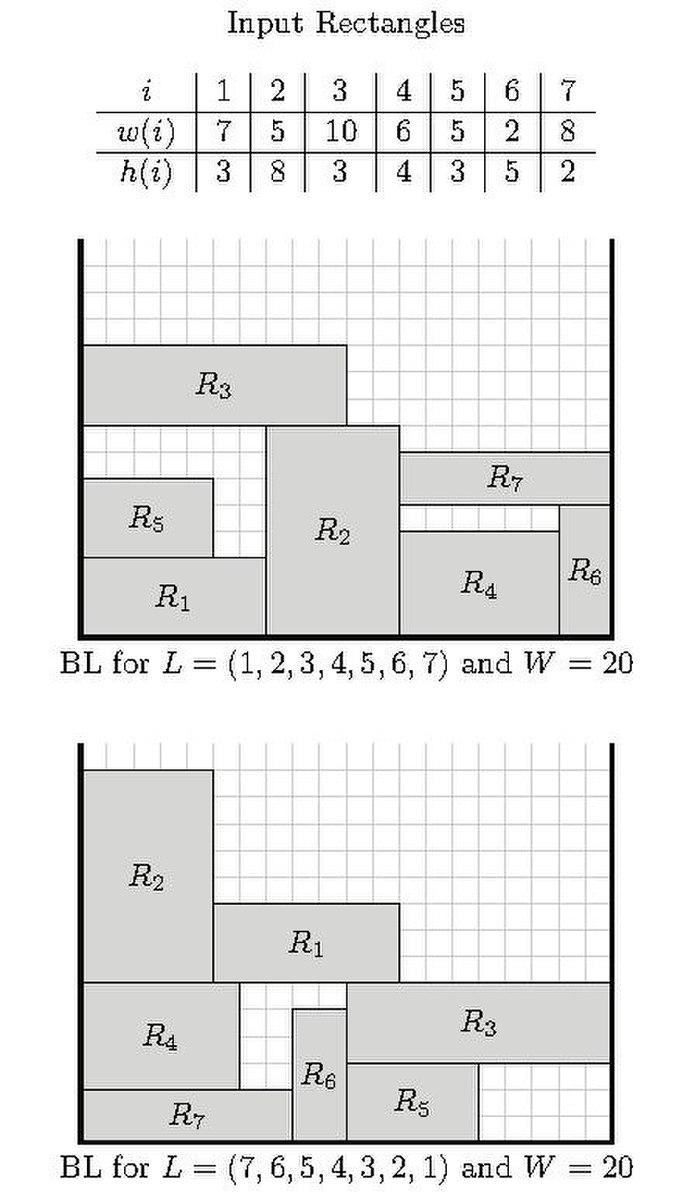
\includegraphics[width=0.3\linewidth]{bl_example.jpg}
\end{center}

Rezaul has collected some related papers into a \href{https://drive.google.com/drive/folders/1EFtuAJ_rq4BaqjXt9jtSUbRW8oqT4RL0?usp=sharing}{google drive}.


\section{Multi-color Strip Packing}

The hardness of this problem follows from strip-packing, when $p = 1$, and in turn bin packing which is NP-Hard.
Last week Lucas showed how to prove the hardness using partitions.

Also, last week we started working on an approximation algorithm
We'll consider two special cases.
\begin{enumerate}
\item There are only 2 programs
\item There are $p$ programs but each includes one task or program
\end{enumerate}

We can prove hardness since when $p = 1$, we have basic strip packing problem
which has been proven to be hard. Last week we considered special case 1.

Lucas said if we had $k$ colors, its trivial to have a $k$-times best approximation.
The idea is to use a bin-packing approximation for one program at a time,
restricted to $\alpha M$ memory, and then stack their solutions.
If the bin-packing approximation has an approximation factor of $A$, then we would 
have a $kA + \epsilon$ approxmation for the multi-color strip-packing problem.

\begin{itemize}
  \item Mayank pointed out this analysis is for completion opt, 
might be stronger for makespan opt?

 \item Rezaul pointed out, why not bin pack all rectangles into $\alpha M$ space?
\end{itemize}

There was some discussion about the exact value of this approximation.
If the first program has  $A \text{Opt}$, second is $2 A \text{Opt}$,
we would get $\frac{k (k +1 )}{2} A \text{Opt}$ in total?

How to do better:
\begin{itemize}
  \item What about shelfing? 
  \item Sorting rectangles some how?
\end{itemize}

Without the $M$ constraint, we can sort rectangles by completion time and doing smaller jobs first will yield optimal completion time. I.e. reduce to $1D$ case.

Another angle discussed was what if all rectangles have the same width? 
When all widths are the same, but not equal to $M$, we could sort the rectangles in non-decreasing order of height
Start arranging left to right and bottom to top.
Undecided if this would be optimial, but it is a natural generalization of the $1D$ problem.
\end{document}







